% $Id: general.tex 9371 2021-08-30 19:54:47Z mskala $

%
% MSK 007 manual introductions
% Copyright (C) 2017, 2021  Matthew Skala
%
% This program is free software: you can redistribute it and/or modify
% it under the terms of the GNU General Public License as published by
% the Free Software Foundation, version 3.
%
% This program is distributed in the hope that it will be useful,
% but WITHOUT ANY WARRANTY; without even the implied warranty of
% MERCHANTABILITY or FITNESS FOR A PARTICULAR PURPOSE.  See the
% GNU General Public License for more details.
%
% You should have received a copy of the GNU General Public License
% along with this program.  If not, see <http://www.gnu.org/licenses/>.
%
% Matthew Skala
% https://northcoastsynthesis.com/
% mskala@northcoastsynthesis.com
%

\chapter{General notes}

This manual documents the MSK~007 Leapfrog VCF, which is a
voltage-controlled filter module for use in a Eurorack modular synthesizer. 
It is a five-pole filter with a leapfrog topology, technically a species of
state-variable filter, with volt/octave tracking; exponential and linear
frequency modulation; and a built-in voltage-controlled amplifier which can
be switched for use on the output or to control feedback.  In
the standard configuration (others may be possible as ``mods''), the
Leapfrog module implements a ``musical near-elliptic'' low-pass curve, with
an extremely sharp cutoff and response peaks at frequencies harmonically
related to the cutoff.

\section{Specifications}

The module's maximum current requirement in ordinary use is 70mA on the
$+$12V supply and 65mA on the $-$12V supply.
Unusual loads on the outputs, including directly-connected headphones or
speakers and so-called ``passive'' modules, may cause the MSK~007 to draw
more than this amount of current.
It does not require $+$5V power.

The input impedance is nominally 100k$\Omega$ for all inputs, varying a
little with control knob positions.  The output impedance is very low, with
current limited by a protection resistor inside an op amp's feedback loop. 
The output is DC coupled.  Shorting any input or output to any fixed voltage
at or between the power rails should be harmless to the module; patching the
MSK~007's output into the output of some other module on the same power
system should be harmless to the MSK~007, though doing that is not
recommended because it is possible the other module may be harmed.

The design target was for a cutoff range from 10Hz to 10kHz, with
oscillation at 0.733 times the cutoff frequency, and V/oct tracking to
within $\pm$5 cents across most if not all of that range.  Those
specifications are not guaranteed, however, and will depend on component
quality, adjustments, and so on.  The first production units tested were
found to have slightly lower limits at both ends, something like 4Hz to
9kHz.

Tracking is
temperature-compensated by an NTC thermistor at and near room temperature,
but not as precisely nor over as wide a temperature range as one might want
for a dedicated oscillator module.
% commented out for future reference - no longer true of latest prototypes
%  The range of the tuning knobs is
% deliberately a little wider than the usable range of the filter, to allow
% compensating control voltage offsets.  \emph{This means there are ``dead
% zones'' at the top and bottom of the tuning range, and these are normal and
% do not indicate a failure in the module.}
The exponential FM input is
nominally also V/octave when set to maximum sensitivity (control knob fully
clockwise), but it is not calibrated and will not be as accurately V/octave
as the main V/octave input.

The VCA control voltage input, at maximum sensitivity (control knob fully
clockwise) is linear with unity gain at roughly 4.8V, normalled to the
equivalent of 5.1V (a little above unity, subject to attenuation) when there
is no cable plugged in.  The gain will increase linearly above unity with
control voltages all the way up to the positive supply at 12V, and it is
safe to use voltages as high as that, though no higher; but output level
limiting, described below, means there may be significant distortion when
using high control voltages.  Negative control voltages cause the VCA to
block signals entirely (zero gain), to the extent possible.

The filter is intended for use with typical Eurorack audio levels of
$\pm$5V (10V peak to peak) but can process considerably higher voltages
with some distortion.  The built-in VCA has soft limiting between 8V and 12V
peak-to-peak (hard limiting at the top of that range), and that defines the
expected maximum audio level under ordinary conditions.  Under extreme
conditions (VCA switched to feedback mode, external control voltage pushing
it beyond unity, a hotter than Eurorack input audio signal, and a lot of
distortion) I have been able to push my prototype unit to 17V peak-to-peak
audio output.  Such use is not damaging \emph{to the MSK~007}; no warranties
are made as to the possible effects on other equipment.

This filter is DC-coupled throughout, so it can be used on control voltages
all the way down to zero frequency.  The tolerances of the analog ICs used
will result in some DC offset appearing on audio signals, and some
feedthrough of control voltage.  An effort has been made in the design to
minimize these effects, but like any other DC-coupled active analog filter,
the MSK~007 will still exhibit them to some degree.

The point of a low-pass filter is to remove part of the signal, and
that implies there will be less signal on the output than on the input.  An
input signal at standard Eurorack level may have significantly less voltage
after passing through the filter, depending on the spectrum and the cutoff
frequency.  This effect occurs with all low-pass filters, but it is stronger
on the MSK~007 than on most others because of the MSK~007's unusually steep
cutoff slope.  The built-in VCA's ability to amplify beyond unity is
intended to help compensate for this effect when desired; but in low-pass
gate applications, the volume loss can be desirable.

This module (assuming a correct build using the recommended components) is
protected against reverse power connection.  It will not function with the
power reversed, but will not suffer or cause any damage.  Some other kinds
of misconnection may possibly be dangerous to the module or the power
supply.

\section{Front panel controls and connections}

Here's a summary of the items on the front panel of the module.

\begin{description}
  \item[TUNING knobs] two of them labelled ``coarse'' and ``fine'':
    these control the basic
    cutoff frequency of the module, which can be modified by input control
    voltages.  The range of the coarse knob is about ten octaves, and that
    of the fine knob about half an octave.

  \item[VCA mode switch] with settings of ``FB'' (to the left) and ``OUT''
    (to the right).  These control whether the built-in VCA controls
    feedback (in which case the module output comes directly from the filter
    core) or output (in which case there is no feedback).  See
    Figure~\ref{fig:vca-block-diagram} for a block diagram.  Note that the
    built-in VCA has a soft-clipping limiter built in, and will result in
    deliberate distortion when used at very high signal levels.

\begin{figure*}
  \centering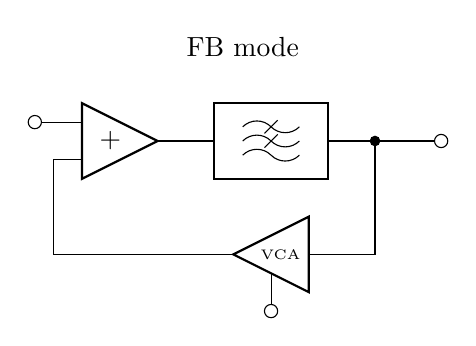
\begin{tikzpicture}[scale=1.2]
    \draw (-2.5,0.2) -- (-2.0,0.2);
    \draw (-0.4,-1.2) -- (-2.3,-1.2) -- (-2.3,-0.2) -- (-2.0,-0.2);
    \draw (-1.2,0) -- (-0.6,0);
    \draw (0.6,0) -- (1.8,0);
    \draw (0,-1.8) -- (0,-1.4);
    \draw (1.1,0) -- (1.1,-1.2) -- (0.4,-1.2);
    \draw[fill=white] (-2.5,0.2) circle[radius=0.07];
    \draw[fill=black] (1.1,0) circle[radius=0.05];
    \draw[fill=white] (1.8,0) circle[radius=0.07];
    \draw[fill=white] (0,-1.8) circle[radius=0.07];
    \draw[thick,fill=white] (-2.0,0.4) -- (-1.2,0) -- (-2.0,-0.4) --cycle;
    \draw[thick,fill=white] (-0.6,-0.4) rectangle (0.6,0.4);
    \draw[thick,fill=white] (0.4,-0.8) -- (-0.4,-1.2) -- (0.4,-1.6) --cycle;
    \draw (-0.3,0.15)
      arc[start angle=135,end angle=45,radius=0.2121]
      arc[start angle=225,end angle=315,radius=0.2121];
    \draw (-0.3,0)
      arc[start angle=135,end angle=45,radius=0.2121]
      arc[start angle=225,end angle=315,radius=0.2121];
    \draw (-0.3,-0.15)
      arc[start angle=135,end angle=45,radius=0.2121]
      arc[start angle=225,end angle=315,radius=0.2121];
    \draw (-0.07,-0.07) -- (0.07,0.07);
    \draw (-0.07,0.08) -- (0.07,0.22);
    \node at (-1.7,0) {$+$};
    \node at (0.1,-1.2) {\tiny VCA};
    \node at (-0.3,1.0) {FB mode};
  \end{tikzpicture}\hspace*{0.7in}%
  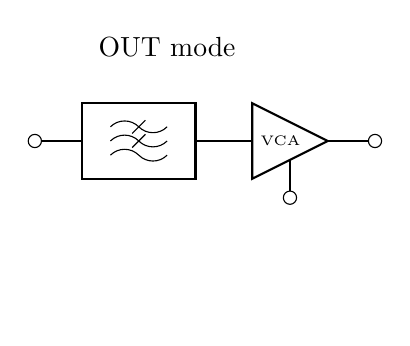
\begin{tikzpicture}[scale=1.2]
    \draw (-1.1,0) -- (2.5,0);
    \draw (1.6,-0.6) -- (1.6,0);
    \draw[fill=white] (-1.1,0) circle[radius=0.07];
    \draw[fill=white] (2.5,0) circle[radius=0.07];
    \draw[fill=white] (1.6,-0.6) circle[radius=0.07];
    \draw[thick,fill=white] (-0.6,-0.4) rectangle (0.6,0.4);
    \draw[thick,fill=white] (1.2,0.4) -- (2.0,0) -- (1.2,-0.4) --cycle;
    \draw (-0.3,0.15)
      arc[start angle=135,end angle=45,radius=0.2121]
      arc[start angle=225,end angle=315,radius=0.2121];
    \draw (-0.3,0)
      arc[start angle=135,end angle=45,radius=0.2121]
      arc[start angle=225,end angle=315,radius=0.2121];
    \draw (-0.3,-0.15)
      arc[start angle=135,end angle=45,radius=0.2121]
      arc[start angle=225,end angle=315,radius=0.2121];
    \draw (-0.07,-0.07) -- (0.07,0.07);
    \draw (-0.07,0.08) -- (0.07,0.22);
    \node at (1.5,0) {\tiny VCA};
    \node at (0.3,1.0) {OUT mode};
    \node at (0,-1.775) {~};
  \end{tikzpicture}\par
  \caption{Simplified block diagram of the module, according to VCA
    mode}\label{fig:vca-block-diagram}
\end{figure*}

  \item[EXP FM knob and jack] This input and attenuator knob add
    exponential FM to the filter cutoff frequency.  Sensitivity is
    approximately 1V/octave with the knob at maximum.  Input voltages
    of $\pm$12V are safe to use, but may not extend the filter's frequencies
    past the range of the tuning knobs.

  \item[LIN FM knob and jack] This input and attenuator knob add linear FM
    to the filter cutoff frequency.  \textit{This is an AC-coupled input and
    DC or very slow AC control voltages will have no effect.}  Sensitivity
    with the knob at maximum is approximately $\pm$100\%\ of the centre
    frequency at $\pm$5V input; it does not support through-zero modulation.

  \item[VCA knob and jack]  This input and attenuator knob control the
    built-in VCA, which in turn either controls feedback or output level
    depending on the VCA mode switch. 
    The control voltage input is normalized to the equivalent of a
    little over 5V, and the
    VCA gives unity gain at about 4.8V.  In feedback mode with no cable
    plugged in, the module will oscillate starting with the knob at about
    half to two thirds of its range.  Note that \textit{the module will
    produce no output} if the switch is set to ``OUT'' and the knob is set
    to minimum, nor if the switch is set to ``OUT'' and there is a cable
    plugged in with a zero control voltage or nothing plugged in at the
    other end.  Voltages in the range $\pm$12V
    are safe to use, but all negative voltages are equivalent to zero;
    voltages higher than 5V give greater than unity voltage gain, but at
    high signal levels will also result in increasing distortion.

  \item[IN jack]  This input is for audio input to the filter.  It is
    intended for standard Eurorack signal levels of $\pm$2.5V, but will
    accept up to $\pm$12V (with distortion likely later in the chain).

  \item[1V/8ve jack]  This is a volt/octave pitch control voltage input.  It
    should be reasonably accurate, and is temperature-compensated, though
    (as appropriate for a filter) it may be less accurate than the best
    dedicated VCOs.

  \item[OUT jack]  This is the audio output from the filter:  either the
    filter core or the VCA depending on the setting of the VCA mode switch.
\end{description}

\section{Source package}

A ZIP archive containing source code for this document and for the module
itself, including things like machine-readable CAD files, is available from 
the Web site at 
\url{https://northcoastsynthesis.com/}.  Be aware that actually building
from source requires some manual steps; Makefiles for GNU Make are provided,
but you may need to manually generate PDFs from the CAD files for inclusion
in the document, make Gerbers from the PCB design, manually edit the .csv
bill of materials files if you change the bill of materials, and so on.

Recommended software for use with the source code includes:
\begin{itemize}
  \item GNU Make;
  \item \LaTeX\ for document compilation;
  \item LaTeX.mk (Danjean and Legrand, not to be confused with other
    similarly-named \LaTeX-automation tools);
  \item Circuit\_macros (for in-document schematic diagrams);
  \item Kicad (electronic design automation);
  \item Qcad (2D drafting); and
  \item Perl (for the BOM-generating script).
\end{itemize}

The kicad-symbols/ subdirectory contains my customised schematic symbol and
PCB footprint libraries for Kicad.  Kicad doesn't normally keep dependencies
like symbols inside a project directory, so on my system, these files
actually live in a central directory shared by many projects.  As a result,
upon unpacking the ZIP file you may need to do some reconfiguration of the
library paths stored inside the project files, in order to allow the symbols
and footprints to be found.  Also, this directory will probably contain some
extra bonus symbols and footprints not actually used by this project,
because it's a copy of the directory shared with other projects.

The package is covered by the GNU GPL, version 3, a copy of which is
included in the file COPYING.

\section{PCBs and physical design}

The enclosed PCB design is for three boards, each
3.90$''$\linebreak[0]$\times$\linebreak[0]2.95$''$, or
99.06mm\linebreak[0]$\times$\linebreak[0]74.93mm.  They are intended to
mount in a stack parallel to the Eurorack panel, held together with M3
machine screws and male-female hex standoff hardware.  See
Figure~\ref{fig:panel-stack}.

\begin{figure}
{\centering
\begin{tikzpicture}[scale=0.1]
  \path[draw=black,dashed,thick] (39.8,-46.95) rectangle (57.8,-26.95);
  \path[draw=black,fill=black!30!white] (-2.0,-64.25) rectangle (0,64.25);
  \path[draw=black,fill=white] (0,-47.45) rectangle (13,-41.45);
  \path[draw=black,fill=white] (0,47.45) rectangle (13,41.45);
  \path[draw=black,fill=blue!50!white] (13,-49.53) rectangle (14.6,49.53);
  \path[draw=black,fill=white] (14.6,-47.45) rectangle (25.6,-41.45);
  \path[draw=black,fill=white] (14.6,47.45) rectangle (25.6,41.45);
  \path[draw=black,fill=blue!50!white] (25.6,-49.53) rectangle (27.2,49.53);
  \path[draw=black,fill=white] (27.2,-47.45) rectangle (38.2,-41.45);
  \path[draw=black,fill=white] (27.2,47.45) rectangle (38.2,41.45);
  \path[draw=black,fill=blue!50!white] (38.2,-49.53) rectangle (39.8,49.53);
  \path[draw=black,fill=white] (39.8,-47.95) rectangle (41.8,-40.95);
  \path[draw=black,fill=white] (39.8,47.95) rectangle (41.8,40.95);
  \path[draw=black,fill=black!10!white] (41.8,-45.95) rectangle (43.8,-42.95);
  \path[draw=black,fill=black!10!white] (41.8,45.95) rectangle (43.8,42.95);
  \node at (6.5,53) {\parbox{13mm}{\centering \small 13mm standoff}};
  \node at (20.1,53) {\parbox{11mm}{\centering \small 11mm standoff}};
  \node at (32.7,53) {\parbox{11mm}{\centering \small 11mm standoff}};
  \node at (13,64) {\small 2mm front panel};
  \node at (26.4,61) {\small 3$\times$ 1.6mm PCBs};
  \draw[>=latex',->,very thick] (13.8,59.7) -- (13.8,50.53);
  \draw[>=latex',->,very thick] (26.4,59.5) -- (26.4,50.53);
  \draw[>=latex',->,very thick] (39.0,59.7) -- (39.0,50.53);
  \node at (48.8,-36.95)
    {\parbox{17mm}{\centering \small 18mm clearance for mated power connector}};
  \draw (57.8,-48) -- (57.8,-64);
  \draw[>=latex',<->,thick] (0,-56) -- (57.8,-56);
  \node[fill=white] at (28.9,-56) {\small $\approx$58mm depth};
\end{tikzpicture}\par}
\caption{Assembled module, side view.}\label{fig:panel-stack}
\end{figure}

\section{Component substitutions}

Most of the components in the circuit are not really critical as to their
identities.  For panel components (the potentiometers, jack sockets, and
DPDT toggle switch), my boards are designed around the components I prefer
to use for quality reasons, including BI Tech conductive-plastic
potentiometers and Lumberg jack sockets.  If you want to substitute cheap,
lower-quality components in a home build, check the PCB design carefully to
make sure it will still work with those components.  The panel-to-board
distance is also carefully chosen, and the recommended components just
barely fit.  Substituting through-panel components means you may need to
take a close look at the physical design to be sure it will still work.

The integrator capacitors (C7, C8, C9, C20, and C21) are
important.\label{pag:integrator-sub}  To achieve an accurate response curve,
they ought to be 470pF $\pm$1\%, and for best audio quality and oscillation
performance across the design range of frequencies, they ought to be at
least good quality film or NP0 types.  Whether people can really hear
differences among capacitor types beyond their objectively-measurable
specifications is a controversial subject.  We can truthfully say that for
best performance in this filter, the capacitors should have close tolerances
and very little loss across the audio spectrum; going any further than that
on capacitor selection \emph{may} only be mumbo-jumbo.
 
North Coast Synthesis Ltd.\ ships polystyrene integration capacitors in our
assembled MSK~007 modules and full kits.  They are top quality, but
expensive, and they require care during soldering.  The PCB includes
alternate through-hole pads for the integration capacitors at 0.2$''$ and
0.6$''$ spacing, and also surface-mount pads, to allow for multiple options
of mounting whatever weird and wonderful capacitors home builders may wish
to substitute.  I used silver mica capacitors in my first prototype; they
work quite well, but are even more expensive than the polystyrene
capacitors, and they may have some loss issues at the lowest audio
frequencies.  Silver mica capacitors are more appropriately used in radio
applications; I would not recommend them here because the less-expensive
polystyrene units are really better.  Good NP0 ceramic capacitors should
work well in this filter, and they are cheaper, but I have not tested them,
and it would probably be necessary to choose surface-mount versions in order
to get the 1\%\ tolerance.  Glass capacitors, sometimes available as
military surplus, possibly with hand-selection to get down to the right
tolerance, would be fun to try.

I recommend two 2N5088 NPN transistors for the exponential converter (Q14
and Q15), as high-quality amplifier transistors likely to be decently
matched without special selection.  I use a third of this same type (Q12) as
a voltage follower in the VCA control voltage processor, in order not to
need yet another distinct component type on the BOM; but really, almost any
typical NPN transistor would be fine for Q12, you could save a few cents by
putting in a 2N3904 there, and you could probably get away with substituting
the exponential transistors with cheaper general purpose types, too.

The Leapfrog VCF uses a lot of PNP discrete transistors in current-source
roles.  I originally designed it using BC557CG transistors in the current
sources.  Those were discontinued shortly before I took the design into
commercial production, and I had to scramble to find a replacement on a
short timeline.  For the first few years of the module's lifetime as a
commercial product, I used PN200A transistors.  In 2021, those were also
discontinued.  As of this writing, I am preparing to switch to SS8550D
transistors for the PNP current sources, and making a lifetime buy to reduce
the risk of future discontinuations.  The SS8550D transistors are a fair
bit more expensive, and they may be overkill for this relatively undemanding
application, but I wanted to make sure there was no quality compromise
involved in making the change.  Really, almost any generic silicon PNP
junction transistor, preferably with high gain, should work.

With any transistor substitution, make sure the pinout is compatible.  Also
be aware that some transistors in TO-92 packages are commonly sold with
``formed'' leads, designed to plug into three holes side by side 0.1$''$
apart, and my boards are designed for use with unformed-lead TO-92 packages,
the leads plugged into a triangular pattern for physical strength.  It is
annoying and requires some care to plug a formed-lead transistor into these
boards; I make an effort to source transistors with unformed leads.

The NTC thermistor used in the control voltage processor (R71) ought to be
Vishay type NTCLE203E3103FB0.  If you cannot get this exact type, you
face a choice of other options:
\begin{itemize}
\item Use some other NTC thermistor with a nominal 10k$\Omega$ resistance at
room temperature, and hope its performance will be close enough;
\item Use a plain metal film 10k$\Omega$ resistor with a very small
temperature coefficient and forfeit temperature compensation;
\item Use a $+$3350ppm/$^\circ$C 22k$\Omega$ PTC ``tempco'' resistor
instead of R75, a plain metal film resistor for R71, and rearrange the
physical design to put R75 in contact with Q14 and Q15, or possibly make
further changes to accomodate a different nominal value of ``tempco''
or reduce the complexity of the resistor network; or
\item Use some other NTC thermistor for R71 and redesign the circuit by
choosing values for R67, R68, R72, and R77, to fit the temperature-to-gain
function as well as possible to the known performance of silicon transistors.
\end{itemize}
Temperature compensation for a filter is usually not critical anyway, so it
may not be a big problem if the performance of this part of the circuit is
not the best possible.

\section{Modification for $\pm$15V power}

The unmodified MSK~007 circuit should work acceptably with $\pm$15V power,
assuming an appropriate substitution or adapter for the Eurorack power
connector itself, and that all components used are rated for the increased
voltage.  Most voltage-critical parts of the circuit are driven by an
internal $+$9V bus, and the regulator for that has plenty of spare power
capacity and should accept $+$15V input without needing any extra heat
sinking.  The DC offset trimmers will need to be adjusted for the voltage
being used.  They and the tuning knobs have range-setting resistors which
are calculated for $\pm$12V, and so will cover a wider range (possibly wider
than is usable, in the case of the coarse tuning knob) unless the range
resistors are changed.  Recommended changes are as follows:

\begin{itemize}
\item R73 (range for coarse tuning knob):  change from 240k$\Omega$ to
  300k$\Omega$
\item R74 (range for fine tuning knob):  change from 4.7M$\Omega$ to
  5.6M$\Omega$
\item R87 (range for core offset trim):  change from 390k$\Omega$ to
  470k$\Omega$.
\item R90 (range for VCA offset trim):  change from 1M$\Omega$ to
  1.2M$\Omega$.
\end{itemize}

\section{Use and contact information}

This module design is released under the GNU GPL, version 3, a copy of which
is in the source code package in the file named \texttt{COPYING}.  One
important consequence of the license is that if you distribute the design to
others---for instance, as a built hardware device---then you are obligated
to make the source code available to them at no additional charge, including
any modifications you may have made to the original design.  Source code for
a hardware device includes without limitation such things as the
machine-readable, human-editable CAD files for the circuit boards and
panels.  You also are not permitted to limit others' freedoms to
redistribute the design and make further modifications of their own.

I sell this and other modules, both as fully assembled products and
do-it-yourself kits, from my Web storefront at
\url{http://northcoastsynthesis.com/}.  Your support of my business is what
makes it possible for me to continue releasing module designs for free. 
Even if you only use the free plans and cannot buy the commercial products I
sell, any assistance you can offer to increasing the profile of North Coast
would be much appreciated.  For instance, you might post photos of your
completed DIY build on your social media.  The latest version of this
document and the associated source files can be found at the North Coast Web
site.

Email should be sent to\\ \url{mskala@northcoastsynthesis.com}.
